\documentclass[cn,11pt]{elegantbook}
% color definitions for code highlighting - also used manually in document (in for example parseString)
\definecolor{comment}{rgb}{1,0.55,0}
\definecolor{string}{rgb}{0.00,0.55,0.55}
\definecolor{identifier}{rgb}{0.10,0.10,0.44}
\definecolor{keyword}{rgb}{0.55,0,0}

\lstset{language=Lisp,
basicstyle=\small\tt,
identifierstyle=\color{identifier},
keywordstyle=\color{keyword}\bfseries,
commentstyle=\color{comment},
showstringspaces=false,
breaklines=true,
morekeywords=define,
basicstyle=\small}

\title{newlisp:优雅的lisp方言}
\subtitle{we love newlisp}

\author{zenghui liu}
\institute{newlisp\funs}
\date{\today}
\version{0.00}

\extrainfo{Victory won\rq t come to us unless we go to it. --- M. Moore}

\logo{figures/newlisp_logo.png}
\cover{cover.jpg}

\begin{document}

\maketitle
\tableofcontents

% \thispagestyle{empty}

\mainmatter
\hypersetup{pageanchor=true}

\chapter{newlisp语言介绍}
newLISP 是一门类 LISP 的,通用用途的脚本语言,
Newlisp将和你以前看到的别的LISP会有很大的差别,所以请将他看成一门全新的语
言。newLISP的最大特点就是自然简洁为应用而生。你不会看到太多的"高级"语法,当然更
不会局限于各种晦涩难懂的教条,当你真正使用newLISP开始工作的时候,你会发
现这是你学过的最简单的语言!

如果你有过编程或者脚本编写的经验,你就会发现newLISP是一个简单易学,功能强大
的脚本语言。既具有传统LISP的优雅,又具有强大实用性:比如正则表达式,网络通信,
Unicode支持,多任务等等。

如果你没有过编程经验,那就更好了。现在就开始newLISP之旅吧。你一定会不虚此行。

经过半个世纪的发展,LISP已经成为了一个语系.无论这些LISP方言之间有多少差别,
他们都遵循了一个至理---"All is Data".

当然newLISP不仅实现了LISP的核心lists,symbols,和lambda表达式.还加入了数组
(arrays),隐式索引(implicit indexing on lists and arrays),动态作用域和词法作用
域(dynamic  and lexical scoping).

毫无疑问newLISP是如今最简洁的LISP,同样也是最易学的LISP.他比Scheme实现起  都小.拥有350个内建函数,不超过260k的大小.内部实现使用大多数UNIX系统中常用的C库
函数.加载速度快,内存消耗小(60k).newLISP比别的流行脚本语言(python...)更快,消耗
更小.

newLISP使用dynamically scope(动态作用域),同时用context(命名空间)完成词法作
用域.context的作用很多.(1) 模块话编程,(2) FOOP(Functional Object Oriented Prog
ramming),(3) 定义保留状态的函数 (4)为关联键值创建hash树.

更多的功能细节请参看手册中的introduction章节:强大的N级嵌套列表操作,方便的- 网络函数(IPV6,IPV4),64系统位支持,PCRE(Perl兼容正则表达式),import(轻松导入任何
共享库),原生的分布式支持,GUI-SERVER跨平台界面库(也可以使用GTK Tcl/Tk 和OpenGL)
 

相关网络资源:
\begin{itemize}
\item 官网:\href{https://newlisp.org/}{https://newlisp.org/}
\item 用户 QQ 群:692108391 
\item 邮件:\email{elegantlatex2e@gmail.com}
\end{itemize}


\section{数值计算}

计算两个整数的最大公约数的函数
\begin{lstlisting}
  (define (MCD a b)
  (let (r (% b a))
  (if (= r 0) a (MCD r a))
  )
  )
\end{lstlisting}

但是我们无法计算3个或更多数字的最大公约数,
为此我们可以使用一个宏处理所有参数

\begin{lstlisting}
  (define (MCD-aux a b)
  (let (r (% b a))
  (if ( = r 0) a (MCD-aux r a))
  )
  )
  (define-macro (MCD)
  (apply MCD-aux (args) 2))
  
\end{lstlisting}

语法: (apply func list [int-reduce])

\subsection{格式}
 
\section{newlisp code patterns}


newLISP是一个类似Lisp语言的、用于一般用途的脚本语言。它具有 LISP 语言所有的魔力,但更容易学习和使用。 newLISP是友好的,快速和简小的。

学习Lisp所收获的是如何自由地表达设计思想

Lisp意为列表处理(List Processing),源自设计者John McCarthy于1960年发表的一篇论文《符号表达式的递归函数及其机器计算》。McCarthy在这篇论文中向我们展示了用一种简单的数据结构S表达式(S-expression)来表示代码和数据,并在此基础上构建一种完整的语言。Lisp语言形式简单、内涵深刻,Paul Graham在《Lisp之根源》中将其对编程的贡献与欧几里德对几何的贡献相提并论。

Lisp的语法基础,Lisp最大的奥秘不在函数式编程,而就在S表达式本身。“S表达式”是程序的一种形,正如“七言”是诗的一种形,“微博”是信息的一种形。人们常认为语法形式不重要,重要的是语言的语义

一门语言能否有效地表达编程者的设计思想取决于其抽象机制的语义表达能力。根据抽象维度的不同,常见的语言抽象机制形成了面向过程、面向对象、函数式、并发式等不同的范式。当我们采用某一种语言,基本上就表示我们已经“面向xxx“了,我们的思维方式和解决问题的手段就会依赖于语言所提供的抽象方式。

无论是面向xxx编程,程序设计都有一条“抽象原则“:what与how解耦,即把语义的声明式表达和实现细节分开,使得程序更容易理解,也更具灵活性。但是,普通语言的问题就在于表达what的手段非常有限,无非是过程、类、接口、函数、Actor等几种语义,这就要求我们在分析建模时必须把领域模型抽象为这些基本语义。但这往往不是许多领域问题最自然的抽象方式

Lisp的柔性与S表达式有着密切的关系。Lisp并不限制你用S表达式来表达什么语义,同样的S表达式语法可以表达各种不同领域的语义,这就是语法和语义解耦。如果说普通语言的刚性源于“语法和语义紧耦合”,那么Lisp的柔性正是源于“语法和语义解耦”!“语法和语义解耦”使得Lisp可以随意地构造各种领域的DSL,而不强制用某一种范式或是领域视角去分析和解决问题。本质上,Lisp编程是一种超越了普通编程范式的范式,这就是Lisp之道:面向语言编程(LOP, Language Oriented Programming)。

LOP范式的基本思想是从问题出发,先创建一门描述领域模型的DSL,再用DSL去解决问题,它具有高度的声明性和抽象性。SQL、make file、CSS等DSL都可以被认为是LOP的具体实例

Lisp采用单一的S表达式语法表达不同的语义,实现了语法和语义解耦。这使得Lisp具有强大的语义构造能力,擅长于构造DSL实现面向语言编程,而宏使得Lisp具有自解释能力,让不同DSL之间的转换游刃有余。进入Lisp的世界应当从理解面向语言编程入门,这是Lisp之道,而函数式编程和宏皆为Lisp之器,以道驭器方为正途。

newLISP是一个类似Lisp语言的、用于一般用途的脚本语言。它具有 LISP 语言所有的魔力,但更容易学习和使用。
newLISP是友好的,快速和简小的

newLISP的最大特点就是语法简单,估计一张纸能说明白最常用的。下面就说几个:

define 是用来定义函数的

newLISP实现了Cilk API, 可以将多个同时运行的进程执行在多处理器或者多核的CPU架构上,已达到并行节省运行时间的目的。

使用spawn和sync函数可以很快的实现。下面是来自newLISP官方文档的例子, 我增加了一行代码

sym 用来保存创建的子进程ID
exp 是子进程启动后运行的表达式,这里我们传递的是函数primes构成的表达式

true 是当父子进程通过send/receive函数通信时才需要设置,一般不需要使用该参数

spawn函数会立刻返回,所以等待子进程返回需要使用sync函数。不过要注意,sync函数返回后,子进程计算结果会保存到sym中。


递归下使用
有一棵任务树,采用广度优先算法递归遍历该树后,为每个节点创建一个进程来执行任务,直到所有节点执行完后,才执行根节点的任务。
由于比较复杂,就不在这里附上我的代码
此次更新主要涉及
\begin{enumerate}
  \item A Modern Built-In API
  \item Regular expressions PCRE 正则表达PCRE
  • \item Pattern matching with match and unify 模式匹配 
  • \item Networking functions: TCP/IP, UDP, HTTP, ICMP 网络函数:TCP/IP, UDP,HTTP, ICMP
  • \item XML and JSON text processing functions xml和json文本处理函数
  • \item Advanced Math and classic Statistics functions 数学和经典统计函数
  • \item Bayesian Statistics functions 贝叶斯统计函数
  • \item Financial functions  
  • \item Date and time functions  时间日期函数
  • \item Fast, unlimited precision integer arithmetic 快速,无限精度整数运算 
  • \item I/O transparent over local files or remote files via HTTP  通过本地文件的io传输或通过http的远程文件传输
  • \item Name spaces (contexts) for programming in modules  模块命令空间(contexts)
  • \item Indexing into nested lists and implicit indexing  列表索引
  • \item Nested associations 
  • \item FOOP Functional Object Oriented Programming. See example  函数式面向对象编程
  • \item Distributed computing support with remote evaluation and HTTP file API  通过api支持分布式计算
  • \item Multi-processing support with Cilk-style API 通过cilk api的多进程支持
  \item Expandable API
  • \item Import functions from C libraries  从c库中导入函数
  • \item Modules for MySQL, SQLite, Zlib, Crypto, Postscript etc. 支持mysql sqlite zlib crypto postscript等模块 
  • \item Document generation support for user written modules: newLISPdoc 文档生成模块newlispdoc
  \item Complete Documentation
  • \item Users Manual and Reference 用户手册和索引
  • \item Cookbook for common solutions Code Patterns in newLISP 
  • \item Introduction (WikiBooks): Introduction to newLISP 介绍图书
  • \item Training videos; see Documentation page 训练材料
  \item Advanced Automatic Memory Management 高级自动内存管理
  • \item ORO memory management oro内存管理
  • \item Synchronous for repeatable processing times in real-time tasks 
  • \item Fast and lower on resources compared to other scripting languages 和其他脚本语言比,快速 资源消耗少
  \item Multiprocessing 多线程编程
  • \item UNIX forks (not on Windows) unit支持forks 
  • \item Semaphores  
  • \item Shared memory 共享内存 
  • \item Local domain UNIX sockets for fast IPC (not on Windows) ipc通信
  • \item Cilk-style multiprocessing API  cilk api 支持
  • \item Actor messaging API for process inter communications actor通信api 
  \item Distributed Computing Support 分布式计算支持
  • \item net-eval function for remote evaluation on multiple network nodes net-eval 多网络节点的远程调用 
  • \item HTTP and net-eval server modes built-in (no code required) 内置http服务
  • \item Most file operations can take URLs  通过urls来操作文件
  \item 64-bit support支持64位系统
  • \item 64-bit standard for integers and some file operations in the standard 32-bit versions 
  • \item LP64 Memory model support makefiles for LINUX, MacOS X and many other UNIX 
  • \item Since 10.5.0 the OSX installer is shipped as a 64-bit application by default 
  \item Small and portable
  • \item Only around 240KB in size on FreeBSD (size depends on compile flavor and platform) 
  • \item Very fast load time for CGI and scripts 
  • \item Uses only the very essential UNIX libs found on the smallest systems 
  • \item Makefiles for macOS , BSDs, LINUX, Windows and many other UNIX 
  \item Embeddable
  • \item Shared library versions for all Platforms (.so, .dylib, .dll) 
  \item International
  • \item Unicode - UTF-8 support compile flavors 
  \item Enterprise
  • \item Well documented 
  • \item Support via responsive community 
  • \item Modules in isolated namespaces 
  • \item Generation of source code API documentation using newLISPdoc utility (similar to javadoc) 
\end{enumerate}


\section{基础}

构建一个list
注意要标记不要求值,比如用‘ 或者list

用函数参数构建一个list
(define-macro (location-file-based-on-modified-time dir-path from-seconds to-seconds)
(println (list from-seconds to-seconds))

\subsection{table-driven模式}
table-drvien,在代码大全中有专门一章介绍,大意是如果条件判断太多,根据不同的条件要执行不同的代码逻辑,用if/else很傻,用switch/case也是一样,用设计模式要写一大堆类。其实有一个更简单的做法,就是key/value类型的数据结构,key为条件,value为执行函数。如果key是整数的话,用一维或者多维数组也可以。

在newlisp中,提供了key/value的接口允许做到table-driven.

\begin{lstlisting}[language=shell,numbers=none,nolol]
  
>(new Tree 'MyTable)
MyTable
>(define (ff) (println "ok"))
(lambda () (println "ok"))
>(MyTable "a" ff)
(lambda () (println "ok"))
>(MyTable "a")
(lambda () (println "ok"))
> ((MyTable "a"))
ok
"ok"
\end{lstlisting}

 
首先定义了一个Tree的子类MyTable,
然后定了一个函数ff
然后将key="a", value=ff的这对保存到MyTable类中。这里和其他语言不一样,是放在MyTable中,而不是其对象中。要注意。
然后就可以用key取出value, 就是ff函数。
如果想立刻运行,用( )执行即可。

字典类型

创建字典
首先Tree是一个namesapce(也就是context),如果想创建一个字典保存key/value结构,需要如下使用
\begin{lstlisting}
(new Tree 'MyTable) 
(MyTable "/home/a.cc" "123:45")
\end{lstlisting}
这样,其实是创建了一个名为MyTable的context,里面用symbol的形式保存了很多key/value的组合。


有个函数,将10进制整数转换成16进制字符串,然后计算长度,如果不够4位,则前面补0.

\begin{lstlisting}
(define (hex-str int-val size)
  (let (v (format "%X" int-val))
    (if (< (length v) size)
    (dotimes (n (- size (length v)))
    (push "0" v))
  v)))
\end{lstlisting}


读取了一个csv文件,统计了每秒能读取读少行
\begin{lstlisting}
(setq t1 (date-value))
(set 'in-file (open "dw_product_dt.csv" "read"))
(setq counter 0)
(while (read-line in-file)
  (inc counter))
(close in-file)
(setq t2 (date-value))
(setq duration (- t2 t1))
(println "totol line number: " counter)
(println (format "read %lld lines per second" (/ counter duration)))
(exit)
 \end{lstlisting}

 \subsection{FFI}
 newlisp可以和其他程序库扩展使用,
 newlisp的import函数, 可以用来导入各种库函数: DLLs (Win32的动态链接库), Linux/Unix 的共享库 (在 Mac OS X 中以 .so 或者 .dylib结尾)。
 

简单的 FFI 扩展接口
newlisp提供了一些扩展函数使用: import, callback , struct , pack 和 unpack . 这些扩展语法只支持使用libffi库构建的newLISP版本。

有了扩展语法, 可以让我们方便地在newLISP中使用C语言中的数据类型,
类似c中函数声明,指定好导入函数的参数类型和返回值就可以,
编码的时候只要将newLISP数据直接传递给调用函数就可以了,剩下转换工作留给ffi。 我们还可以将newLISP函数注册为callback(回调函数),提供给导入函数调用。
扩展语法虽然也支持浮点数结构,不过不建议使用浮点数,因为不是所以的系统平台都支持。
扩展API会根据不同的CPU架构,自动将转换后类型的数据做对齐操作。 具体的扩展语法请看用户手册。

下面介绍的API大部分都可使用。

首先 用C写共享库,编译库文件,newlisp调用库即可
用C写共享库
接下来演示如何在Win32 and Linux/Unix 上用C语言编写和编译共享库.

\begin{lstlisting}
#include <stdio.h>
#include <stdlib.h>
#include <ctype.h>
 
int foo1(char * ptr, int number)
{
  printf("the string: %s the number: %d\n", ptr, number);
  return(10 * number);
}
 
char * foo2(char * ptr, int number)
{
  char * upper;
  printf("the string: %s the number: %d\n", ptr, number);
  upper = ptr;
  while(*ptr) { *ptr = toupper(*ptr); ptr++; }
  return(upper);
}
\end{lstlisting}

在UNIX上编译共享库
On Mac OS X and Linux/Unix 使用下面的方法编译 testlib.so :

gcc testlib.c -shared -o testlib.so

testlib.so 构建的时候做了 cdecl 转换(NIX默认)。
testlib.dll构造的时候做了 stdcall 转换(Win32 默认)。

构建完毕库文件后,在newlisp直接import函数
\begin{lstlisting}
> (import "/home/newlisp/testlib.so" "foo1")
foo1 <6710118F>
 
> (import "/home/newlisp/testlib.so" "foo2")
foo2 <671011B9>
 
> (foo1 "hello" 123)
the string: hello the number: 123
1230
 
> (foo2 "hello" 123)
the string: hello the number: 123
4054088
 
> (get-string (foo2 "hello" 123))
the string: hello the number: 123
"HELLO"
>
\end{lstlisting}
注意: foo2 返回的 4054088 字符串的内存地址. 要用get-string才能读取字符串内容. 因为newLISP会根据系统自动判断库函数的调用类型, 在WIN32下,默认的函数调用类型是 stdcall,所以如果你在 WIN32 上调用的库是 cdecl 的, 就必须用 cdecl 关键字申明.

'C' 结构和 'C' 字符串一样都可以通过指针操作访问,'C' 结构中的成员可以使用 get-string, get-int or get-char 访问. 下面来看样例:
\begin{lstlisting}
  typedef struct mystruc
   {
   int number;
   char * ptr;
   } MYSTRUC;
 
MYSTRUC * foo3(char * ptr, int num )
   {
   MYSTRUC * astruc;
   astruc = malloc(sizeof(MYSTRUC));
   astruc->ptr = malloc(strlen(ptr) + 1);
   strcpy(astruc->ptr, ptr);
   astruc->number = num;
   return(astruc);
 }
\end{lstlisting}

可以使用下面的方法访问结构成员(不是唯一的方法):
\begin{lstlisting}
 > (set 'astruc (foo3 "hello world" 123))
4054280
 
> (get-string (get-integer (+ astruc 4)))
"hello world"
 
> (get-integer astruc)
123
\end{lstlisting}
foo3 返回的是结构 astruc 的地址. (+ astruc 4)是字符串的地址, 在32位OS里 'C' 语言的一个整数4个字节的内存(MYSTRUC 的 int number). 字符串通过 get-string 访问.
如上所示, 如果某些导入函数申请了内存却没有释放. 就必须用 libc 里的函数 free 来释放这些申请的数据,
如果传递给导入函数的数据,是newLISP数据的引用, 就不需要手工释放内存了(因为newLISP会做)
\begin{lstlisting}
  (import "/usr/lib/libc.so" "free")

(free astruc) ; astruc contains memory address of allocated structure
\end{lstlisting}

参数传递
data Type	newLISP call	C function call
integer	(foo 123)	foo(int number)
double float	(foo 1.234)	foo(double number)
float	(foo (flt 1.234))	foo(float number)
string	(foo "Hello World!")	foo(char * string)
integer array	(foo (pack "d d d" 123 456 789))	foo(int numbers[])
float array	(foo (pack "f f f" 1.23 4.56 7.89))	foo(float[])
double array	(foo (pack "lf lf lf) 1.23 4.56 7.89)	foo(double[])
string array	(foo (pack "lu lu lu" "one" "two" "three")))	foo(char * string[])


提取返回值
data Type	newLISP to extract return value	C return
integer	(set 'number (foo x y z))	return(int number)
double float	n/a - only 32bit returns, use double float pointer instead	not available
double float ptr	(set 'number (get-float (foo x y z)))	return(double * numPtr)
float	not available	not available
string	(set 'string (get-string (foo x y z)	return(char * string)
integer array	(set 'numList (unpack "ld ld ld" (foo x y z)))	return(int numList[])
float array	(set 'numList (unpack "f f f" (foo x y z)))	return(float numList[])
double array	(set 'numList (unpack "lf lf lf") (foo x y z)))	return(double numList[])
string array	(set 'stringList (map get-string (unpack "ld ld ld" (foo x y z))))	return(char * string[])


Floats 和 doubles 只能通过地址操作(任何get- 函数操作的都是地址).
如果返回的是数组,则必须知道数组长度才能提取. 例子假设的长度都是三.
所有的 pack 和 unpack 格式化字符之间也可以没有空格,不过那样可读性会很差(比如(unpack "fldb" (foo x y z)) 是不是很蛋疼)
"ld" 和 "lu" 可以互换(这里有疑惑,地址是可以但是数据...), 但是16位的 "u" 和 "d" 可能会产生不同的结果, 因为从 16 到 32 位是正数增长.

pack 和 unpack 可以在大端和小端之间切换.


编写封装库
import 有时候无法导入库. 这是因为库没有遵循正规的 cdecl 调用,将所有的参数压入堆栈. 比如将 Mac OS X 运行在老式的 PPC CPUs 上, 默认安装的OpenGL库将无法使用.

这时可以写一个专门的封装库将 cdecl 调用转换成目标库的调用方式.

\begin{lstlisting}
  /* wrapper.c - demo for wrapping library function
 
compile:
    gcc -m32 -shared wrapper.c -o wrapper.so
or:
    gcc -m32 -bundle wrapper.c -o wrapper.dylib
 
usage from newLISP:
 
    (import "./wrapper.dylib" "wrapperFoo")
 
    (define (glFoo x y z)
        (get-float (wrapperFoo 5 (float x) (int y) (float z))) )
 
 (glFoo 1.2 3 1.4) => 7.8
 
*/
 
#include <stdio.h>
#include <stdarg.h>
 
 
/* the glFoo() function would normally live in the library to be
   wrapped, e.g. libopengl.so or libopengl.dylib, and this
   program would link to it.
   For demo and test purpose the function has been included in this
   file
*/
 
double glFoo(double x, int y, double z)
    {
    double result;
 
    result = (x + z) * y;
 
    return(result);
    }
 
/* this is the wrapper for glFoo which gets imported by newLISP
   declaring it as a va-arg function guarantees 'cdecl'
   calling conventions on most architectures
*/
 
double * wrapperFoo(int argc, ...)
    {
    va_list ap;
    double x, z;
    static double result;
    int y;
 
    va_start(ap, argc);
 
    x = va_arg(ap, double);
    y = va_arg(ap, int);
    z = va_arg(ap, double);
 
    va_end(ap);
 
    result = glFoo(x, y, z);
    return(&result);
  }
\end{lstlisting}

为扩展库注册回调函数
newLISP的内建函数 callback 可以获取用户定义函数的地址, 并将他注册成库函数的回调函数:
\begin{lstlisting}
  (define (keyboard key x y)
  (if (= (& key 0xFF) 27) (exit)) ; exit program with ESC
  (println "key:" (& key 0xFF) " x:" x  " y:" y))

  (glutKeyboardFunc (callback 1 'keyboard))
\end{lstlisting}


利用共享库执行代码
第一个例子我们用newLISP 调用自己的共享库函数 newlispEvalStr:
\begin{lstlisting}
(import "/usr/lib/newlisp.so" "newlispEvalStr")
(get-string (newlispEvalStr "(+ 3 4)")) →  "7\n"
\end{lstlisting}

newlispEvalStr 的返回值总是一个字符串指针. 必须用 get-string 获得其中的内容. 所有的结果,就算是数字,都会以字符串(加换行符)的形式返回.如果不需要输出可以用 silent 函数屏蔽. 要得到数字,可以通过 int 或者 float 转换.

要传递多行代码必须用 [cmd], [/cmd]:


newLISP has two FFI APIs. The simple API needs no type specifiers but is limited to integers and pointers. The extended API can specify types for return values and parameters and can also be used for floats and structs.

\begin{lstlisting}
  (import "libc.dylib" "strdup")
  (println (get-string (strdup "hello world")))

  ; or extended FFI interface on Mac OSX
  (import "libc.dylib" "strdup" "char*" "char*")
  (println (strdup "hello world"))
\end{lstlisting}

\section{应用}

\subsection{系统}
监控Linux进程
判断进程是否存活,如果不是,则重新启动, 监控进程的cpu和memory占用情况.

在用newlisp创建多个进程模拟客户端进行测试的时候,关闭是个问题,下面的脚本很方便的杀掉所有newlisp进程

\begin{lstlisting}[lisp]
#!/usr/local/bin/newlisp

(set 'r (exec "pidof newlisp"))
(dolist (l r)
  (exec (append "kill " l)))
\end{lstlisting}

远程运行newlisp代码

newlisp 提供一个简单的mapreduce方式,利用net-eval函数,向远程运行newlisp服务进程的机器发起调用

首先服务器启动进程

newlisp -l -c -d 4711 &

-l 代表记录日志,默认打印到终端
-c 是
-d 是链接之前保存状态,一个效果就是后续请求必须等待前面的请求完成才能发出

\begin{lstlisting}
  ; calculate primes in a range
(define (primes from to)
    (local (plist)
    (for (i from to)
        (if (= 1 (length (factor i)))
        (push i plist -1)))
plist))
 
; start child processes
(set 'start (time-of-day))
 
(spawn 'p1 (primes 1 1000000))
(spawn 'p2 (primes 1000001 2000000))
(spawn 'p3 (primes 2000001 3000000))
(spawn 'p4 (primes 3000001 4000000))
 
; wait for a maximum of 60 seconds for all tasks to finish
(sync 60000) ; returns true if all finished in time
; p1, p2, p3 and p4 now each contain a lists of primes
\end{lstlisting}
例子中将1到4000000分成4个部分,传递给primes (搜索素数的)子进程,通过 spawn (会立即返回)并行启动,处理完的数据放到4个symbol里. 最后调用 sync 阻塞等待子进程60秒,直到子进程全部返回并存储到4个symbol里.

用newlisp cilk API可以实现多进程通信。在实际应用中,父进程发送消息给多个子进程,使得父进程可以专注于自己的工作,把一些额外的工作交给子进程去完成,做到对父进程任务无阻塞的效果。

1. 父子进程消息交换

父进程通过send发送消息,子进程通过receiv接收消息,使用了循环和等待,一直反复接收消息。

2. spawn执行后,'result不会立刻得到结果,值为nil。这不是错误,是newlisp这么设计的。需要等到(sync)调用后才能获得子进程返回的结果。

\subsection{网站开发}

为什么用newlisp开发网站?

1. 并不是一定要高性能
因为很多应用都是网站的方式发布,易于升级,而并不是很多网站一定要具备高性能要求,一定要用C++写网站。

2. 脚本式编程容易理解和维护

Java, 太重了,做个网站搞上那么多开源框架。罗嗦的要命,脚本式编程容易修改,不存在编译时运行时的差别。ruby, php, python有它繁荣的道理,newlisp也是脚本语言。

3. 后端比重不大,学习成本不高

在web 2.0之后的年代,前端编程才是主要的工作量,后端解决一个基本的网页渲染,数据库读取,提供REST API即可。所以后端的代码比重不大,因此对于我这种前后端开发都很熟悉的人来讲,newlisp只是一个后端解决方案,学习成本不高,工作量不大。

resp api
 
\subsection{XML相关}

用注释生成文档
@module 定义模块
@description 描述
@loaction 文件位置
@version 版本
@author 作者
@example 例子
@note
@syntax 语法
@throw 抛出异常
@note 笔记

最后运行newlispdoc file.lsp
\begin{lstlisting}
;; file.lsp

;; @module file
;; @description file module provides some file operations on both Ubuntu and Windows
;; @location file.lsp
;; @version 1.0
;; @author Dean Chen
;; @example
;; (let ((test-dir1 (append (real-path) file:file-seperator "a")) (test-dir2 (append (real-path) file:file-seperator "b")))
;;   (make-dir test-dir1)
;;   (make-dir test-dir2)
;;   (if (directory? test-dir1)
;;       (begin
;; 	(unless (catch (file:copy-folder test-dir1 test-dir2) 'result)
;; 		(println (append "catch error: " result))
;; 		(println "test copy-folder failed"))
;; 	(file:remove-folder test-dir1)
;; 	(file:remove-folder test-dir2))))
(context 'file)

;; @syntax (file:init)
;; @throw Throw error if environment variable NEWLISP_ARMORY_HOME does not exist or is invalid
;; @throw Throw error if OS is not Windows or UBuntu
;; @note init function will be called automatically when loading file.lsp module, don't call it manually
(define (init)
  (unless (env "NEWLISP_ARMORY_HOME")
	  (throw-error "NEWLISP_ARMORY_HOME does not exist"))
  (unless (file? (env "NEWLISP_ARMORY_HOME"))
	  (throw-error "NEWLISP_ARMORY_HOME points to a non-existing file"))
  (unless (directory? (env "NEWLISP_ARMORY_HOME"))
	  (throw-error "NEWLISP_ARMORY_HOME points to a file instead of directory"))
  (set 'file-folder (append (env "NEWLISP_ARMORY_HOME") "/codes/file"))
  (if
   (= ostype "Linux") (load (append file-folder "/file_ubuntu.lsp"))
   (= ostype "Win32") (load (append file-folder "/file_win.lsp"))
   (throw-error (append "file tool doesn't support this OS for now, ostype:" ostype))
   ))
 \end{lstlisting}
 \subsection{模块化编程}

 构造一个程序 当你的代码比较多或者各个代码文件之间充斥着大量重复代码的时候,

 就必须把这些冗余的代码划分进一个个不同的代码模块(否则你很可能写出"九阴真经").
   newLISP中使用context来创建模块, 也就是命名空间. 命名空间将各个模块之间的词法隔离开.
   这样各模块可以拥有相同名字的变量而不冲突.

一个模块文件包含数据库访问代码.

用context封装数据
前面的例子都是使用函数将数据封装在不同命名空间中. 在 generator 的例子中 acc 用来保存状态. 在 fibo 的例子中用 mem 来保存增长的列表. 两个例子里,函数和变量结合在了一起. 下面的例子中直接将数据赋值给默认函数,而不使用函数(其实function is data):

用引用传递对象
当默认函数被作为某个函数的参数调用的时候, 默认函数会通过引用传递. 这意味这传递给函数的参数是原始数据, 而不是列表或者字符串的拷贝. 在传递庞大的数据的时候这个特性非常有用:

\subsection{局部变量}

循环函数中的局部变量,
所有的循环函数 doargs, dolist, dostring, dotimes, dotree 和 for 都使用局部变量。 在循环结构内部,每一次循环,局部变量都能获得不同的值。
但是在出了循环以后,循环内部的局部变量将消失。
let, define, 和 lambda 是另一种申明局部变量的方法:

用 let 和 local 申明局部变量
let 是一种常见的申明本地变量的方法.
你可以通过免安装的方式使用本模板,也可以通过安装模板的方式使用。


\section{在线使用模板}
考虑到用户的在线合作需求,我们把三套模板全部上传到 \href{https://www.overleaf.com/}{Overleaf} 上了,网络通畅的用户可以直接通过 Overleaf 在线使用我们的模板。这样的好处是无需安装 \TeX{} Live 2019,可以随时随地访问自己的文件。查找模板,请在 Overleaf 模板库里面搜索 \lstinline{elegantlatex} 即可,你也可以直接访问\href{https://www.overleaf.com/latex/templates?addsearch=elegantlatex}{搜索结果}。选择适当的模板之后,将其 \lstinline{Open as Template},即可把模板存到自己账户下,然后可以自由编辑以及与别人一起协作。更多关于 Overleaf 的介绍和使用,请参考 Overleaf 的\href{https://www.overleaf.com/learn}{官方文档}。

\begin{remark}
Overleaf 上,中文需要使用 \lstinline{XeLaTeX} 进行编译,英文可以使用 \lstinline{PDFLaTeX} 与 \lstinline{XeLaTeX} 进行编译。
\end{remark}

\section{用户作品计划}
Elegant\LaTeX{} 系列模板从创立至今已经有 8 年了,我们的模板也受到了很多用户的喜爱,在此,为了促进模板用户之间的交流,了解用户需求,完善本模板,我们将建立一个区域专门展示用户的文档,包括但不限于 Github 和官网等。如果你愿意将自己的作品展示出来,请邮件或者其他方式联系我们。如果自己代码已经传到 Github 或者 Gitee 等网站,可以提供对应网址。

\section{关于提交}
出于某些因素的考虑,Elegant\LaTeX{} 项目自 2019 年 5 月 20 日开始,\textbf{不再接受任何非作者预约性质的提交}(pull request)!如果你想改进模板,你可以给我们提交 issues,或者可以在遵循协议(LPPL-1.3c)的情况下,克隆到自己仓库下进行修改。

\section{协作人员招募}
招募 Elegant\LaTeX{} 的协作人员,没有工资。工作内容:翻译 Elegant\LaTeX{} 系列模板相关的文稿(中文->英文),维护模板的 wiki(主要涉及 Markdown 语法),如果有公众号文稿写作经历的话,也可以帮忙写微信稿。本公告长期有效。

\section{致谢}
2019 年 5 月 20 日,ElegantBook 模板在 Github 上的 star 数达到了 100,并且 21 日上了 Github 网站 \TeX{} 语言的\href{https://github.com/trending/tex?since=daily}{日趋势榜单}。这对于 Elegant\LaTeX{} 系列模板都是一个里程碑!

在此特别感谢 China\TeX{} 以及 \href{http://www.latexstudio.net/}{\LaTeX{} 工作室}对于本系列模板的大力宣传与推广。\LaTeX{} 工作室网站上有很多精彩的帖子和精致的模板,欢迎大家去挖掘里面的宝藏。这也是国内最全面的 \LaTeX{} 相关的网站。

特别感谢 \href{https://github.com/muzimuzhi}{muzimuzhi} 对于模板的完善。

如果你喜欢我们的模板,你可以在 Github 上收藏我们的模板。
\begin{figure}[htbp]
\centering
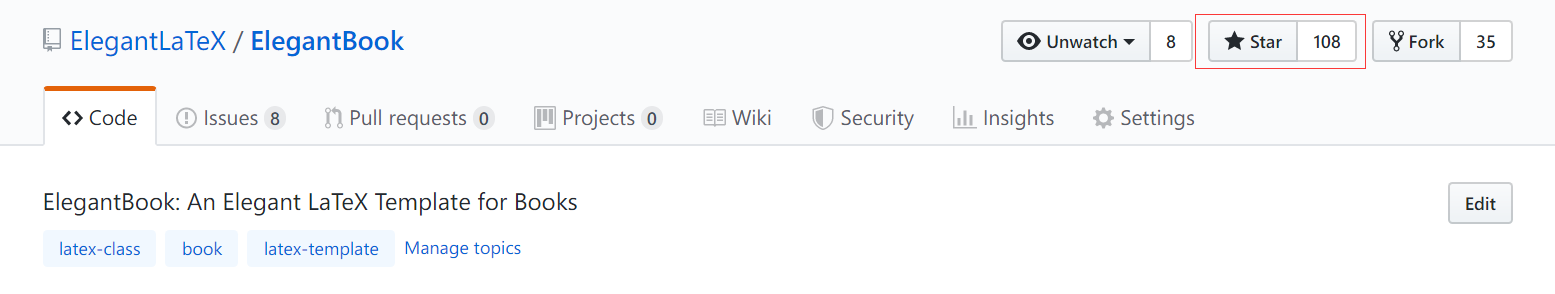
\includegraphics[width=\textwidth]{star.png}
\caption{一键三连求赞}
\end{figure}

之前我们模板从未发布过捐赠/打赏信息,近期有用户反映他们对我们模板非常喜爱,想打赏没有支付码,不禁感叹,这世道变了啊,还有主动打赏的,那么我们就“勉为其难”地发布我们的打赏二维码吧!

\begin{figure}[htbp]
\centering

\includegraphics[width=0.5\textwidth]{donate.jpg}
\end{figure}

赞赏费用的使用解释权归 Elegant\LaTeX{} 所有,并且不接受监督,请自愿理性打赏,10 元以上的赞赏,我们将列入捐赠榜,谢谢各位金主!

\begin{table}[htbp]
  \centering
  \caption{捐赠榜}
    \begin{tabular}{cccc}
    \toprule
    捐赠者   & 金额 & 时间 & 渠道 \\
    \midrule
    Lerh  & 10 元  & 2019/5/15 & 微信 \\
    越过地平线 & 10 元    & 2019/5/15 & 微信 \\
	大熊 &  20 元 & 2019/5/27 & 微信 \\
    \bottomrule
    \end{tabular}%
\end{table}%

再次感谢大家对于模板的喜爱!

\chapter{code patterns}

本模板基于基础的 book 文类,所以 book 的选项对于本模板也是有效的。
默认编码为 UTF-8,推荐使用 \TeX{} Live 编译
。本文编写环境为 Win10 (64bit) + \TeX{} Live 2019,支持 \lstinline{PDFLaTeX} 以及 \lstinline{XeLaTeX} 编译。


\section{语言模式}
\subsection{列表的嵌套层}

计算list的最大嵌套深度
\begin{lstlisting}  
(define (nesting lst prev (t 0))
  (if (= lst prev)
      t
      (nesting (flat lst 1) lst (inc t))))

;;(nesting '(a (((b c (d)))) (e) ((f)) g))
\end{lstlisting}

这里使用了 flat 和 inc 两个函数

\subsection{最大乘积子表}

本模板内含两套语言环境,改变语言环境会改变图表标题的引导词(图,表),
文章结构词(比如目录,参考文献等),以
及定理环境中的引导词(比如定理,引理等)。不同语言模式的启用如下:
\begin{lstlisting}
\documentclass[cn]{elegantbook} 
\documentclass[lang=cn]{elegantbook}
\end{lstlisting}

\begin{remark}
只有中文环境(\lstinline{lang=cn})才可以输入中文。另外如果抄录环境(\lstinline{lstlisting})中有中文字符,请务必使用 \lstinline{XeLaTeX} 编译。
\end{remark}

\section{设备选项}
最早我们在 ElegantNote 模板中加入了设备选项(\lstinline{device}),后来,我们觉得这个设备选项的设置可以应用到 ElegantBook 中\footnote{不过因为 ElegantBook 模板封面图片的存在,在修改页面设计时,需要对图片进行裁剪。},而且 Book 一般内容比较多,如果在 iPad 上看无需切边,放大,那用户的阅读体验将会得到巨大提升。你可以使用下面的选项将版面设置为 iPad 设备模式\footnote{默认为 normal 模式,也即 A4 纸张大小。}
\begin{lstlisting}
\documentclass[pad]{elegantbook} %or
\documentclass[device=pad]{elegantbook}
\end{lstlisting}

\section{颜色主题}
本模板内置 5 组颜色主题,分别为 \textcolor{structure1}{\lstinline{green}}\footnote{为原先默认主题。}、\textcolor{structure2}{\lstinline{cyan}}、\textcolor{structure3}{\lstinline{blue}}(默认)、\textcolor{structure4}{\lstinline{gray}}、\textcolor{structure5}{\lstinline{black}}。另外还有一个自定义的选项  \lstinline{nocolor}。调用颜色主题 \lstinline{green} 的方法为 
\begin{lstlisting}
\documentclass[green]{elegantbook} %or
\documentclass[color=green]{elegantbook}
\end{lstlisting}

\begin{table}[htbp]
\caption{ElegantBook 模板中的颜色主题\label{tab:color thm}}
\centering
\begin{tabular}{ccccccc}
\toprule
	        & \textcolor{structure1}{green} 
	        & \textcolor{structure2}{cyan} 
	        & \textcolor{structure3}{blue}
	        & \textcolor{structure4}{gray} 
	        & \textcolor{structure5}{black} 
	        & 主要使用的环境\\
\midrule
structure & \makecell{{\color{structure1}\rule{1cm}{1cm}}}
				& \makecell{{\color{structure2}\rule{1cm}{1cm}}}
				& \makecell{{\color{structure3}\rule{1cm}{1cm}}} 
				& \makecell{{\color{structure4}\rule{1cm}{1cm}}} 
				& \makecell{{\color{structure5}\rule{1cm}{1cm}}} 
				& chapter \ section \ subsection \\

main      & \makecell{{\color{main1}\rule{1cm}{1cm}}}
				& \makecell{{\color{main2}\rule{1cm}{1cm}}}
				& \makecell{{\color{main3}\rule{1cm}{1cm}}}
				& \makecell{{\color{main4}\rule{1cm}{1cm}}}
				& \makecell{{\color{main5}\rule{1cm}{1cm}}}
				& definition \ exercise \ problem \\

second    & \makecell{{\color{second1}\rule{1cm}{1cm}}}
				& \makecell{{\color{second2}\rule{1cm}{1cm}}}
				& \makecell{{\color{second3}\rule{1cm}{1cm}}}
				& \makecell{{\color{second4}\rule{1cm}{1cm}}}
				& \makecell{{\color{second5}\rule{1cm}{1cm}}}
				& theorem \ lemma \ corollary\\

third     & \makecell{{\color{third1}\rule{1cm}{1cm}}}
				& \makecell{{\color{third2}\rule{1cm}{1cm}}}
				& \makecell{{\color{third3}\rule{1cm}{1cm}}}
				& \makecell{{\color{third4}\rule{1cm}{1cm}}}
				& \makecell{{\color{third5}\rule{1cm}{1cm}}}
				& proposition\\
\bottomrule
\end{tabular}
\end{table}

如果需要自定义颜色的话请选择 \lstinline{nocolor} 选项或者使用 \lstinline{color=none},然后在导言区定义 structurecolor、main、second、third 颜色,具体方法如下:
\begin{lstlisting}
\definecolor{structurecolor}{RGB}{0,0,0}
\definecolor{main}{RGB}{70,70,70}    
\definecolor{second}{RGB}{115,45,2}    
\definecolor{third}{RGB}{0,80,80}   
\end{lstlisting}


\section{章标题显示风格}

本模板内置 2 套\textit{章标题显示风格},包含 \lstinline{hang}(默认)与 \lstinline{display} 两种风格,区别在于章标题单行显示(\lstinline{hang})与双行显示(\lstinline{display}),本说明使用了 \lstinline{hang}。调用方式为
\begin{lstlisting}
\documentclass[hang]{elegantbook} %or
\documentclass[titlestyle=hang]{elegantbook}
\end{lstlisting}

\section{数学环境简介}

在我们这个模板中,我们定义了两种不同的定理模式 \lstinline{mode},包括简单模式(\lstinline{simple})和炫彩模式(\lstinline{fancy}),默认为 \lstinline{fancy} 模式,不同模式的选择为
\begin{lstlisting}
\documentclass[simple]{elegantbook} %or
\documentclass[mode=simple]{elegantbook}
\end{lstlisting}

本模板定义了四大类环境

\begin{itemize}
\item \textit{定理类环境},包含标题和内容两部分,全部定理类环境的编号均以章节编号。根据格式的不同分为 3 种
   \begin{itemize}
      \item \textcolor{main}{\textbf{definition}} 环境,颜色为 \textcolor{main}{main};
      \item \textcolor{second}{\textbf{theorem、lemma、corollary}} 环境,颜色为 \textcolor{second} {second};
      \item \textcolor{third}{\textbf{proposition}} 环境,颜色为 \textcolor{third}{third}。
   \end{itemize}
\item \textit{示例类环境},有 \textbf{example、exercise、problem} 环境(对应于例,练习,例题),自动编号,编号以章节为单位。
\item \textit{证明类环境},有 \textbf{proof、note} 环境,特点是,有引导符或者结尾符,\textbf{note} 环境有引导符号,\textbf{proof} 环境有证明完毕符号。
\item \textit{结论类环境},有 \textbf{conclusion、assumption、property,remark、solution} 环境\footnote{本模板还添加了一个 result 选项,用于隐藏 \lstinline{solution} 和 \lstinline{proof} 环境,默认为显示(\lstinline{result=answer}),隐藏使用 \lstinline{result=noanswer}。},三者均以粗体的引导词为开头,和普通段落格式一致。
\end{itemize}

\subsection{定理类环境的使用}
由于本模板使用了 \lstinline{tcolorbox} 宏包来定制定理类环境,所以和普通的定理环境的使用有些许区别,定理的使用方法如下:
\begin{lstlisting}
\begin{theorem}{theorem name}{label}
The content of theorem.
\end{theorem}
\end{lstlisting}

第一个必选项 \lstinline{theorem name} 是定理的名字,第二个必选项 \lstinline{label} 是交叉引用时所用到的标签,交叉引用的方法为 \verb|\ref{thm:label}|。请注意,交叉引用时必须加上前缀 \lstinline{thm:}。

其他相同用法的定理类环境有:

\begin{table}[htbp]
   \centering
   \caption{定理类环境}
     \begin{tabular}{llll}
     \toprule
     环境名 & 标签名 & 前缀 & 交叉引用 \\
     \midrule
     definition & label & def   & \lstinline|\ref{def:label}| \\
     theorem & label & thm   & \lstinline|\ref{thm:label}| \\
     lemma & label & lem   & \lstinline|\ref{lem:label}| \\
     corrlary & label & cor   & \lstinline|\ref{cor:label}| \\
     proposition & label & pro   & \lstinline|\ref{pro:label}| \\
     \bottomrule
     \end{tabular}%
   \label{tab:theorem-class}%
 \end{table}%
 

\subsection{其他环境的使用}
其他三种环境没有选项,可以直接使用,比如 \lstinline{example} 环境的使用方法与效果:
\begin{lstlisting}
\begin{example}
   This is the content of example environment.
\end{example}
\end{lstlisting}

\begin{example}
This is the content of example environment.
\end{example}


这几个都是同一类环境,区别在于

\begin{itemize}
   \item 示例环境(example)、练习(exercise)与例题(problem)章节自动编号;
   \item 注意(note)环境有提醒引导符,证明(proof)环境有证明结束符;
   \item 结论(conclusion)等环境都是普通段落环境,引导词加粗。
\end{itemize}

\section{装饰物}

本模板为章节后的装饰物(base)添加了隐藏选项,有 \lstinline{show} 和 \lstinline{hide} 两个选项。
\begin{lstlisting}
\documentclass[hide]{elegantbook} %or
\documentclass[base=hide]{elegantbook}
\end{lstlisting}

\section{封面和徽标}

本模板使用的封面图片来源于 \href{https://pixabay.com/en/tea-time-poetry-coffee-reading-3240766/}{pixabay.com}\footnote{感谢 China\TeX{} 提供免费图源网站,另外还推荐 \href{https://www.pexels.com/}{pexels.com}。},图片完全免费,可用于任何场景。封面图片的尺寸为 $1280 \times 1024$, 更换图片的时候请\textbf{严格}按照封面图片尺寸进行裁剪。推荐一个免费的在线图片裁剪网站 \href{https://www.befunky.com/create/crop-photo/}{befunky.com}。

本文用到的 Logo 比例为 1:1,也即正方形图片,在更换图片的时候请选择合适的图片进行替换。

\section{列表环境}
本模板借助于 \lstinline{tikz} 定制了 \lstinline{itemize} 和 \lstinline{enumerate} 环境,其中 \lstinline{itemize} 环境修改了 3 层嵌套,而 \lstinline{enumerate} 环境修改了 4 层嵌套(仅改变颜色)。示例如下\\[2ex]
\begin{minipage}[b]{0.49\textwidth}
\begin{itemize}
   \item first item of nesti;
   \item second item of nesti;
   \begin{itemize}
      \item first item of nestii;
      \item second item of nestii;
      \begin{itemize}
         \item first item of nestiii;
         \item second item of nestiii.
      \end{itemize}   
   \end{itemize}
\end{itemize}
\end{minipage}
\begin{minipage}[b]{0.49\textwidth}
\begin{enumerate}
   \item first item of nesti;
   \item second item of nesti;
   \begin{enumerate}
      \item first item of nestii;
      \item second item of nestii;
      \begin{enumerate}
         \item first item of nestiii;
         \item second item of nestiii.
      \end{enumerate}   
   \end{enumerate}
\end{enumerate}
\end{minipage}

\section{参考文献}

此模板使用了 \hologo{BibTeX} 来生成参考文献,在中文示例中,使用了 \lstinline{gbt7714} 宏包。参考文献示例:\cite{en1,en2,en3} 使用了中国一个大型的 P2P 平台(人人贷)的数据来检验男性投资者和女性投资者在投资表现上是否有显著差异。

你可以在谷歌学术,Mendeley,Endnote 中获得文献条目(bib item),然后把它们添加到 \lstinline{reference.bib} 中。在文中引用的时候,引用它们的键值(bib key)即可。注意需要在编译的过程中添加 \hologo{BibTeX} 编译。如果你想添加未引用的文献,可以使用
\begin{lstlisting}[frame=single]
\nocite{EINAV2010,Havrylchyk2018} %or include some bibitems
\nocite{*} %include all the bibitems
\end{lstlisting}

本模板还添加了 \lstinline{cite=numbers} 和 \lstinline{cite=authoryear} 两个参考文献选项,用于设置参考文献格式的设置,默认为 \lstinline{numbers}。据我们所知,理工科类一般使用 \lstinline{numbers},而文科类使用 \lstinline{authoryear} 比较多,所以我们将 \lstinline{numbers} 作为默认格式。如果需要改为  \lstinline{authoryear} ,可以使用
\begin{lstlisting}
\documentclass[cite=authoryear]{elegantbook} %or
\documentclass[authoryear]{elegantbook}
\end{lstlisting}

\section{添加序章}

如果你想在第一章前面添序章,不改变原本章节序号,可以在第一章内容前面使用 
\begin{lstlisting}
\chapter*{Introduction}
\addcontentsline{toc}{chapter}{Introduction} 
\markboth{Introduction}{} 
The content of introduction.
\end{lstlisting}

\section{章节摘要}
模板新增了一个章节摘要环境(introduction),使用示例
\begin{lstlisting}
\begin{introduction}
	\item Definition of Theorem
	\item Ask for help
	\item Optimization Problem
	\item Property of Cauchy Series
	\item Angle of Corner
\end{introduction}
\end{lstlisting}
效果如下:
\begin{introduction}
	\item Definition of Theorem
	\item Ask for help
	\item Optimization Problem
	\item Property of Cauchy Series
	\item Angle of Corner
\end{introduction}

环境的标题文字可以通过这个环境的可选参数进行修改,修改方法为:
\begin{lstlisting}
\begin{introduction}[Brief Introduction]
...
\end{introduction}
\end{lstlisting}


\section{章后习题}
前面我们介绍了例题和练习两个环境,这里我们再加一个,章后习题(\lstinline{problemset})环境,用于在每一章结尾,显示本章的练习。使用方法如下

\begin{lstlisting}
\begin{problemset}
	\item exercise 1
	\item exercise 2
	\item exercise 3
\end{problemset}
\end{lstlisting}


效果如下:
\begin{problemset}
	\item exercise 1
	\item exercise 2
	\item exercise 3
\end{problemset}

\begin{remark}
如果你想把 \lstinline{problemset} 环境的标题改为其他文字,你可以类似于 introduction 环境修改 problemset 的可选参数。
\end{remark}

\chapter{ElegantBook 写作示例}

\begin{introduction}
\item 积分定义~\ref{def:int}
\item Fubini 定理~\ref{thm:fubi}
\item 最优性原理~\ref{pro:max}
\item 柯西列性质~\ref{property:cauchy}
\item 韦达定理
\end{introduction}

\section{Lebesgue 积分}
在前面各章做了必要的准备后,本章开始介绍新的积分。在 Lebesgue 测度理论的基础上建立了 Lebesgue 积分,其被积函数和积分域更一般,可以对有界函数和无界函数统一处理。正是由于 Lebesgue 积分的这些特点,使得 Lebesgue 积分比 Riemann 积分具有在更一般条件下的极限定理和累次积分交换积分顺序的定理,这使得 Lebesgue 积分不仅在理论上更完善,而且在计算上更灵活有效。

Lebesgue 积分有几种不同的定义方式。我们将采用逐步定义非负简单函数,非负可测函数和一般可测函数积分的方式。

由于现代数学的许多分支如概率论、泛函分析、调和分析等常常用到一般空间上的测度与积分理论,在本章最后一节将介绍一般的测度空间上的积分。

\subsection{积分的定义}

我们将通过三个步骤定义可测函数的积分。首先定义非负简单函数的积分。以下设 $E$ 是 $\mathcal{R}^n$ 中的可测集。


\begin{definition}{可积性}{int}
设 $ f(x)=\sum\limits_{i=1}^{k} a_i \chi_{A_i}(x)\oint_{a}^b\ointop_{a}^b\prod_{i=1}^n$ 是 $E$ 上的非负简单函数,其中 $\{A_1,A_2,\ldots,A_k\}$ 是 $E$ 上的一个可测分割,$a_1,a_2,\ldots,a_k$ 是非负实数。定义 $f$ 在 $E$ 上的积分为 $\int_{a}^b f(x)$
\begin{equation}
   \label{inter}
   \int_{E} f dx = \sum_{i=1}^k a_i m(A_i) \pi \alpha\beta\sigma\gamma\nu\xi\epsilon\varepsilon. \oint_{a}^b\ointop_{a}^b\prod_{i=1}^n
\end{equation}
一般情况下 $0 \leq \int_{E} f dx \leq \infty$。若 $\int_{E} f dx < \infty$,则称 $f$ 在 $E$ 上可积。
\end{definition}

一个自然的问题是,Lebesgue 积分与我们所熟悉的 Riemann 积分有什么联系和区别?在 4.4 在我们将详细讨论 Riemann 积分与 Lebesgue 积分的关系。这里只看一个简单的例子。设 $D(x)$ 是区间 $[0,1]$ 上的 Dirichlet 函数。即 $D(x)=\chi_{Q_0}(x)$,其中 $Q_0$ 表示 $[0,1]$ 中的有理数的全体。根据非负简单函数积分的定义,$D(x)$ 在 $[0,1]$ 上的 Lebesgue 积分为
\begin{equation}
   \label{inter2}
   \int_0^1 D(x)dx = \int_0^1 \chi_{Q_0} (x) dx = m(Q_0) = 0
\end{equation}
即 $D(x)$ 在 $[0,1]$ 上是 Lebesgue 可积的并且积分值为零。但 $D(x)$ 在 $[0,1]$ 上不是 Riemann 可积的。



有界变差函数是与单调函数有密切联系的一类函数。有界变差函数可以表示为两个单调递增函数之差。与单调函数一样,有界变差函数几乎处处可导。与单调函数不同,有界变差函数类对线性运算是封闭的,它们构成一线空间。练习题 \ref{exer:43} 是一个性质的证明。

\begin{exercise}\label{exer:43}
设 $f \notin\in L(\mathcal{R}^1)$,$g$ 是 $\mathcal{R}^1$ 上的有界可测函数。证明函数
\begin{equation}
   \label{ex:1}
   I(t) = \int_{\mathcal{R}^1} f(x+t)g(x)dx \quad t \in \mathcal{R}^1
\end{equation}
是 $\mathcal{R}^1$ 上的连续函数。
\end{exercise}

\begin{problem}
即 $D(x)$ 在 $[0,1]$ 上是 Lebesgue 可积的并且积分值为零。但 $D(x)$ 在 $[0,1]$ 上不是 Riemann 可积的。
\end{problem}

\begin{solution}
即 $D(x)$ 在 $[0,1]$ 上是 Lebesgue 可积的并且积分值为零。但 $D(x)$ 在 $[0,1]$ 上不是 Riemann 可积的。
\end{solution}

\begin{theorem}{Fubini 定理}{fubi} 
(1)若 $f(x,y)$ 是 $\mathcal{R}^p\times\mathcal{R}^q$ 上的非负可测函数,则对几乎处处的 $x\in \mathcal{R}^p$,$f(x,y)$ 作为 $y$ 的函数是 $\mathcal{R}^q$ 上的非负可测函数,$g(x)=\int_{\mathcal{R}^q}f(x,y) dy$ 是 $\mathcal{R}^p$ 上的非负可测函数。并且
\begin{equation}
   \label{eq:461}
   \int_{\mathcal{R}^p\times\mathcal{R}^q} f(x,y) dxdy=\int_{\mathcal{R}^p}\left(\int_{\mathcal{R}^q}f(x,y)dy\right)dx.
\end{equation}
(2)若 $f(x,y)$ 是 $\mathcal{R}^p\times\mathcal{R}^q$ 上的可积函数,则对几乎处处的 $x\in\mathcal{R}^p$,$f(x,y)$ 作为 $y$ 的函数是 $\mathcal{R}^q$ 上的可积函数,并且 $g(x)=\int_{\mathcal{R}^q}f(x,y) dy$ 是 $\mathcal{R}^p$ 上的可积函数。而且~\ref{eq:461} 成立。
\end{theorem}

\begin{note}
在本模板中,引理(lemma),推论(corollary)的样式和定理~\ref{thm:fubi} 的样式一致,包括颜色,仅仅只有计数器的设置不一样。
\end{note}

我们说一个实变或者复变量的实值或者复值函数是在区间上平方可积的,如果其绝对值的平方在该区间上的积分是有限的。所有在勒贝格积分意义下平方可积的可测函数构成一个希尔伯特空间,也就是所谓的 $L^2$ 空间,几乎处处相等的函数归为同一等价类。形式上,$L^2$ 是平方可积函数的空间和几乎处处为 0 的函数空间的商空间。

\begin{proposition}{最优性原理}{max}
如果 $u^*$ 在 $[s,T]$ 上为最优解,则 $u^*$ 在 $[s, T]$ 任意子区间都是最优解,假设区间为 $[t_0, t_1]$ 的最优解为 $u^*$ ,则 $u(t_0)=u^{*}(t_0)$,即初始条件必须还是在 $u^*$ 上。
\end{proposition}

我们知道最小二乘法可以用来处理一组数据,可以从一组测定的数据中寻求变量之间的依赖关系,这种函数关系称为经验公式。本课题将介绍最小二乘法的精确定义及如何寻求点与点之间近似成线性关系时的经验公式。假定实验测得变量之间的 $n$ 个数据,则在平面上,可以得到 $n$ 个点,这种图形称为 “散点图”,从图中可以粗略看出这些点大致散落在某直线近旁, 我们认为其近似为一线性函数,下面介绍求解步骤。

\begin{figure}[htbp]
	\centering
	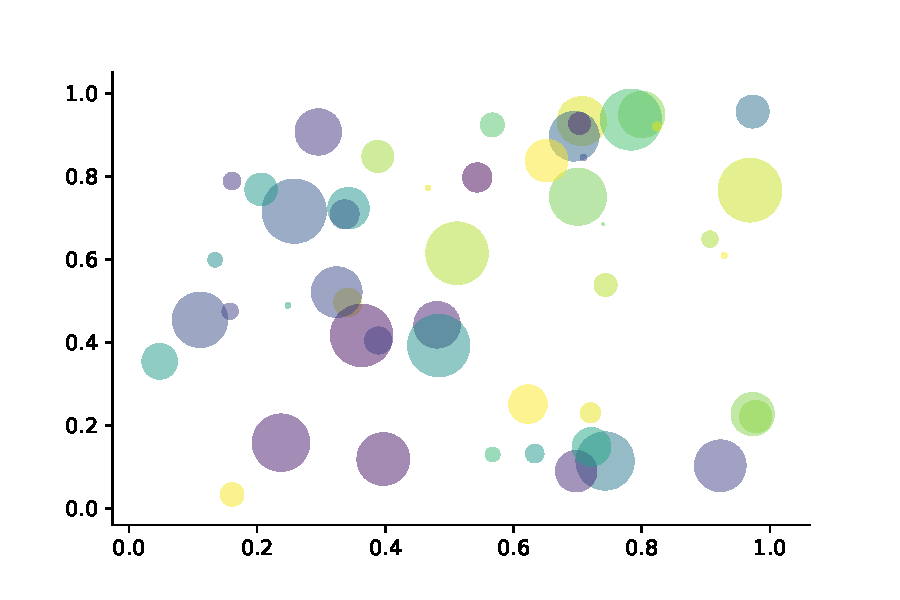
\includegraphics[width=0.6\textwidth]{scatter.pdf}
	\caption{散点图示例 $\hat{y}=a+bx$ \label{fig:scatter}}
\end{figure}

以最简单的一元线性模型来解释最小二乘法。什么是一元线性模型呢?监督学习中,如果预测的变量是离散的,我们称其为分类(如决策树,支持向量机等),如果预测的变量是连续的,我们称其为回归。回归分析中,如果只包括一个自变量和一个因变量,且二者的关系可用一条直线近似表示,这种回归分析称为一元线性回归分析。如果回归分析中包括两个或两个以上的自变量,且因变量和自变量之间是线性关系,则称为多元线性回归分析。对于二维空间线性是一条直线;对于三维空间线性是一个平面,对于多维空间线性是一个超平面。

\begin{property}\label{property:cauchy}
柯西列的性质
\begin{enumerate}
\item $\{x_k\}$ 是柯西列,则其子列 $\{x_k^i\}$ 也是柯西列。
\item $x_k\in \mathcal{R}^n$,$\rho(x,y)$ 是欧几里得空间,则柯西列收敛,$(\mathcal{R}^n,\rho)$ 空间是完备的。
\end{enumerate}
\end{property}

\begin{conclusion}
回归分析(regression analysis) 是确定两种或两种以上变量间相互依赖的定量关系的一种统计分析方法。运用十分广泛,回归分析按照涉及的变量的多少,分为一元回归和多元回归分析;按照因变量的多少,可分为简单回归分析和多重回归分析;按照自变量和因变量之间的关系类型,可分为线性回归分析和非线性回归分析。
\end{conclusion}

\begin{problemset}
\item 设 $A$ 为数域 $K$ 上的 $n$ 级矩阵。证明:如果 $K^n$ 中任意非零列向量都是 $A$ 的特征向量,则 $A$ 一定是数量矩阵。
\item 证明:不为零矩阵的幂零矩阵不能对角化。
\item 设 $A = (a_{ij})$ 是数域 $K$ 上的一个 $n$ 级上三角矩阵,证明:如果 $a_{11} = a_{22} = \cdots = a_{nn}$,并且至少有一个 $a_{kl} \not = 0 (k < l)$,则 $A$ 一定不能对角化。
\end{problemset}

\chapter{旁注}
在 3.08 版本,我们加入了旁注(边注)等设置以及 \lstinline{\elegantpar} 命令,不过目前处于测试阶段。如果你想整个文档都加入旁注,一般的方法是,重新设置旁注的大小。本模板加入了一个旁注选项 \lstinline{marginpar},如果加入旁注 \lstinline{marginpar=margintrue},则会减少版芯两边的宽度(减少至 1.5cm),如果不加入旁注 \lstinline{marginpar=marginfalse}(默认),则维持两边距离不变。旁注选项仅对 \lstinline{device=normal} 试用,pad 模式并不支持。

旁注命令可以使用 \LaTeX{} 自带的 \lstinline{\marginpar} 命令或者 \lstinline{marginnote}  宏包的  \lstinline{\marginnote}  命令,旁注的使用,请参考维基百科:\href{https://en.wikibooks.org/wiki/LaTeX/Footnotes_and_Margin_Notes#Margin_Notes}{旁注}或者 \LaTeX {}书籍。

本模板还添加了一个 \lstinline{\elegantpar} 命令,需要注意的是,由于这个命令使用了 TikZ 中的层叠效果(overlay),所以为了得到正确的旁注显示,你需要多次编译(3 次)。\lstinline{\elegantpar} 命令的效果如下。

%\setlength{\marginparwidth}{2.5cm}
Lorem ipsum dolor sit amet, consectetur adipisicing elit, sed do eiusmod
tempor incididunt ut labore et \elegantpar{dolore magna aliqua}{This is Beautiful the elegantpar Style for English Text}. Ut enim ad minim veniam,
quis nostrud exercitation ullamco laboris nisi ut aliquip ex ea commodo
consequat. Duis aute irure dolor in reprehenderit in voluptate velit esse
cillum dolore eu fugiat nulla pariatur. Excepteur sint occaecat cupidatat non
proident, sunt in culpa qui officia deserunt mollit anim id est laborum.

\begin{equation}
a^{2}+b^{2} = \elegantpar{c^{2}}{勾股定理
\begin{equation*}a^2+b^2=c^2\end{equation*}}
\end{equation}
 
 若夫日出而林霏开,云归而岩穴暝,晦明变化者,山间之朝暮也。野芳发而幽香,佳木秀而繁阴,风霜高洁,水落而石出者,山间之四时也。朝而往,暮而归,四时之景不同,而乐亦无穷也。 
 
 至于负者歌于途,行者休于树,前者呼,后者应,\elegantpar{伛偻提携}{指搀扶着走的小孩子},往来而不绝者,滁人游也。临溪而渔,溪深而鱼肥。酿泉为酒,泉香而酒洌;山肴野蔌,杂然而前陈者,太守宴也。宴酣之乐,非丝非竹,射者中,弈者胜,觥筹交错,起坐而喧哗者,众宾欢也。苍颜白发,颓然乎其间者,太守醉也。$2\elegantpar{x}{方程的解与数学符号的选择无关}=3$。

 \chapter{FAQ}
 \begin{custom}{问题}
   什么是newlisp,能用来做什么呢?
 \end{custom}

   newlisp 是类lisp的脚本语言,它能做脚本语言所能做的:比如互联网编程,系统管理,处理文本数据
   调用其他程序等。newlisp是为那些对lisp的优美和强悍的表达能力而着迷的人准备的,同时它也非常容易让人学习

\chapter{常见问题集}

begin{custom}{问题}
有没有办法章节用“第一章,第一节,(一)”这种?
\end{custom}

\begin{solution}
你可以修改模板中对于章节的设置,利用 ctex 宏集的 \lstinline{\zhnumber} 命令可以把计数器的数字形式转为中文。
\end{solution}


\begin{custom}{问题}
3.07 版本的 cls 的 natbib 加了numbers 编译完了没变化,群主设置了不可更改了?
\end{custom}

\begin{solution}
3.07 中在 \lstinline{gbt7714} 宏包使用时,加入了 \lstinline{authoryear} 选项,这个使得 \lstinline{natbib} 设置了 \lstinline{numbers} 也无法生效。3.08 版本中,模板增加了 \lstinline{numbers} 和 \lstinline{authoryear} 文献选项,你可以参考前文设置说明。
\end{solution}

\begin{custom}{问题}
大佬,我想把正文字体改为亮色,背景色改为黑灰色。
\end{custom}

\begin{solution}
页面颜色可以使用 \lstinline{\pagecolor} 命令设置,文本命令可以参考\href{https://tex.stackexchange.com/questions/278544/xcolor-what-is-the-equivalent-of-default-text-color}{这里}进行设置。
\end{solution}

\begin{custom}{问题}
\lstinline{! LaTeX Error: Unknown option `scheme=plain' for package `ctex'.}
\end{custom}

\begin{solution}
你用的 C\TeX{} 套装吧?这个里面的 \lstinline{ctex} 宏包已经是已经是 10 年前的了,与本模板使用的 \lstinline{ctex} 宏集有很大区别。不建议 C\TeX{} 套装了,请卸载并安装 \TeX{} Live 2019。
\end{solution}

\begin{custom}{问题}
我该使用什么版本?
\end{custom}

\begin{solution}
请务必使用\href{https://github.com/ElegantLaTeX/ElegantBook/releases}{最新正式发行版},发行版间不定期可能会有更新(修复 bug 或者改进之类),如果你在使用过程中没有遇到问题,不需要每次更新\href{https://github.com/ElegantLaTeX/ElegantBook/archive/master.zip}{最新版},但是在发行版更新之后,请尽可能使用最新版(发行版)!最新发行版可以在 Github 或者 \TeX{} Live 2019 内获取。
\end{solution}


\begin{custom}{问题}
我该使用什么编辑器?
\end{custom}

\begin{solution}
你可以使用 \TeX{} Live 2019 自带的编辑器 \TeX{}works 或者使用 \TeX{}studio,\TeX works 的自动补全,你可以参考我们的总结 \href{https://github.com/EthanDeng/texworks-autocomplete}{\TeX works 自动补全}。推荐使用 \TeX{} Live 2019 + \TeX Studio。我自己用 VS Code 和 Sublime Text,相关的配置说明,请参考 \href{https://github.com/EthanDeng/vscode-latex}{\LaTeX{} 编译环境配置:Visual Studio Code 配置简介} 和 \href{https://github.com/EthanDeng/sublime-text-latex}{Sublime Text 搭建 \LaTeX{} 编写环境}。
\end{solution}


\begin{custom}{问题}
您好,我们想用您的 ElegantBook 模板写一本书。关于机器学习的教材,希望获得您的授权,谢谢您的宝贵时间。
\end{custom}

\begin{solution}
模板的使用修改都是自由的,你们声明模板来源以及模板地址(github 地址)即可,其他未尽事宜按照开源协议 LPPL-1.3c。做好之后,如果方便的话,可以给我们一个链接,我把你们的教材放在 ElegantLaTeX 用户作品集里。
\end{solution}

\begin{custom}{问题}
我想要原来的封面!
\end{custom}

\begin{solution}
我们计划在未来版本加入封面选择,让用户可以选择旧版封面。
\end{solution}

\begin{custom}{问题}
我想修改中文字体!
\end{custom}

\begin{solution}
首先,我们{\heiti 强烈建议你不要去修改字体}!如果你一定坚持修改字体,请在 \lstinline{newtxtext} 宏包加载前加入中文字体设置(\lstinline{xeCJK} 宏包)。如果你选择自定义字体,请设置好 \lstinline{\kaishu},\lstinline{\heiti} 等命令,否则会报错。如果你看不懂我现在说的,请停止你的字体自定义行为。
\end{solution}

\begin{custom}{问题}
请问交叉引用是什么?
\end{custom}

\begin{solution}
本群和本模板适合有一定 \LaTeX{} 基础的用户使用,新手请先学习 \LaTeX{} 的基础,理解各种概念,否则你将寸步难行。
\end{solution}

\begin{custom}{问题}
定义等环境中无法使用加粗命令么?
\end{custom}

\begin{solution}
是这样的,默认中文并没加粗命令,如果你想在定义等环境中使用加粗命令,请使用 \lstinline{\heiti} 等字体命令,而不要使用 \lstinline{\textbf}。或者,你可以将 \lstinline{\textbf} 重新定义为 \lstinline{\heiti}。英文模式不存在这个问题。
\end{solution}

\begin{custom}{问题}
代码高亮环境能用其他语言吗?
\end{custom}

\begin{solution}
可以的,ElegantBook 模板用的是 \lstinline{listings} 宏包,你可以在环境之后加上语言,全局语言修改请使用 \lstinline{\lstset} 命令,更多信息请参考宏包文档。
\end{solution}


\begin{custom}{问题}
群主,什么时候出 Beamer 的模板(主题),ElegantSlide 或者 ElegantBeamer?
\end{custom}

\begin{solution}
这个问题问的人比较多,我这里给个明确的答案。由于 Beamer 中有一个很优秀的主题 \href{https://github.com/matze/mtheme}{Metropolis}。我觉得在我们找到非常好的创意之前不会发布正式的 Beamer 主题,如果你非常希望得到 Elegant\LaTeX{} “官方”的主题,请在用户 QQ 群内下载我们测试主题 PreElegantSlide(未来不一定按照这个制作)。正式版制作计划在 2020 年之后。
\end{solution}

\begin{custom}{问题}
群主好棒,想嫁!
\end{custom}

\begin{solution}
我取向正常!
\end{solution}


\nocite{*} 

\bibliography{reference}

\appendix
\chapter{基本数学工具}

本附录包括了计量经济学中用到的一些基本数学,我们扼要论述了求和算子的各种性质,研究了线性和某些非线性方程的性质,并复习了比例和百分数。我们还介绍了一些在应用计量经济学中常见的特殊函数,包括二次函数和自然对数,前 4 节只要求基本的代数技巧,第 5 节则对微分学进行了简要回顾;虽然要理解本书的大部分内容,微积分并非必需,但在一些章末附录和第 3 篇某些高深专题中,我们还是用到了微积分。

\section{求和算子与描述统计量}

\textbf{求和算子} 是用以表达多个数求和运算的一个缩略符号,它在统计学和计量经济学分析中扮演着重要作用。如果 $\{x_i: i=1, 2, \ldots, n\}$ 表示 $n$ 个数的一个序列,那么我们就把这 $n$ 个数的和写为:

\begin{equation}
\sum_{i=1}^n x_i \equiv x_1 + x_2 +\cdots + x_n
\end{equation}


\chapter{newlisp 命令列表}


\section{List processing, flow control, and integer arithmetic}

\begin{itemize}
  \item +, -, *, /, %     integer arithmetic
  \item ++                increment integer numbers
 \item --                decrement integer numbers
 \item <, >, =           compares any data type: less, greater, equal
  \item <=, >=, !=        compares any data type: less-equal, greater-equal, not-equal
:                 constructs a context symbol and applies it to an object
and               logical and
append            appends lists ,arrays or strings to form a new list, array or string
apply             applies a function or primitive to a list of arguments
args              retrieves the argument list of a function or macro expression
assoc             searches for keyword associations in a list
begin             begins a block of functions
bigint            convert a number to big integer format
bind              binds variable associations in a list
case              branches depending on contents of control variable
catch             evaluates an expression, possibly catching errors
chop              chops elements from the end of a list
clean             cleans elements from a list
collect           repeat evaluating an expression and collect results in a list
cond              branches conditionally to expressions
cons              prepends an element to a list, making a new list
constant          defines a constant symbol
count             counts elements of one list that occur in another list
curry             transforms a function f(x, y) into a function fx(y)
define            defines a new function or lambda expression
define-macro      defines a macro or lambda-macro expression
def-new           copies a symbol to a different context (namespace)
difference        returns the difference between two lists
doargs            iterates through the arguments of a function
dolist            evaluates once for each element in a list
dostring          evaluates once for each character in a string
dotimes           evaluates once for each number in a range
dotree            iterates through the symbols of a context
do-until          repeats evaluation of an expression until the condition is met
do-while          repeats evaluation of an expression while the condition is true
dup               duplicates a list or string a specified number of times
ends-with         checks the end of a string or list against a key of the same type
eval              evaluates an expression
exists            checks for the existence of a condition in a list
expand            replaces a symbol in a nested list
explode           explodes a list or string
extend            extends a list or string
first             gets the first element of a list or string
filter            filters a list
find              searches for an element in a list or string
flat              returns the flattened list
fn                defines a new function or lambda expression
for               evaluates once for each number in a range
for-all           checks if all elements in a list meet a condition
if                evaluates an expression conditionally
index             filters elements from a list and returns their indices
intersect         returns the intersection of two lists
lambda            defines a new function or lambda expression
last              returns the last element of a list or string
length            calculates the length of a list or string
let               declares and initializes local variables
letex             expands local variables into an expression, then evaluates
letn              initializes local variables incrementally, like nested lets
list              makes a list
local             declares local variables
lookup            looks up members in an association list
map               maps a function over members of a list, collecting the results
match             matches patterns against lists; for matching against strings, see find and regex
member            finds a member of a list or string
not               logical not
nth               gets the nth element of a list or string
or                logical or
pop               deletes and returns an element from a list or string
pop-assoc         removes an association from an association list
push              inserts a new element into a list or string
quote             quotes an expression
ref               returns the position of an element inside a nested list
ref-all           returns a list of index vectors of elements inside a nested list
rest              returns all but the first element of a list or string
replace           replaces elements inside a list or string
reverse           reverses a list or string
rotate            rotates a list or string
select            selects and permutes elements from a list or string
self              Accesses the target object inside a FOOP method
set               sets the binding or contents of a symbol
setf setq         sets contents of a symbol or list, array or string reference
set-ref           searches for an element in a nested list and replaces it
set-ref-all       searches for an element in a nested list and replaces all instances
silent            works like begin but suppresses console output of the return value
slice             extracts a sublist or substring
sort              sorts the members of a list
starts-with       checks the beginning of a string or list against a key of the same type
swap              swaps two elements inside a list or string
unify             unifies two expressions
unique            returns a list without duplicates
union             returns a unique list of elements found in two or more lists.
unless            evaluates an expression conditionally
until             repeats evaluation of an expression until the condition is met
when              evaluates a block of statements conditionally
while             repeats evaluation of an expression while the condition is true
\end{itemize}
String and conversion functions
===============================
address           gets the memory address of a number or string
bigint            convert a number to big integer format
bits              translates a number into binary representation
char              translates between characters and ASCII codes
chop              chops off characters from the end of a string
dostring          evaluates once for each character in a string
dup               duplicates a list or string a specified number of times
ends-with         checks the end of a string or list against a key of the same type
encrypt           does a one-time–pad encryption and decryption of a string
eval-string       compiles, then evaluates a string
explode           transforms a string into a list of characters
extend            extends a list or string
find              searches for an element in a list or string
find-all          returns a list of all pattern matches found in string
first             gets the first element in a list or string
float             translates a string or integer into a floating point number
format            formats numbers and strings as in the C language
get-char          gets a character from a memory address
get-float         gets a double float from a memory address
get-int           gets a 32-bit integer from a memory address
get-long          gets a long 64-bit integer from a memory address
get-string        gets a string from a memory address
int               translates a string or float into an integer
join              joins a list of strings
last              returns the last element of a list or string
lower-case        converts a string to lowercase characters
member            finds a list or string member
name              returns the name of a symbol or its context as a string
nth               gets the nth element in a list or string
pack              packs newLISP expressions into a binary structure
parse             breaks a string into tokens
pop               pops from a string
push              pushes onto a string
regex             performs a Perl-compatible regular expression search
regex-comp        pre-compiles a regular expression pattern
replace           replaces elements in a list or string
rest              gets all but the first element of a list or string
reverse           reverses a list or string
rotate            rotates a list or string
select            selects and permutes elements from a list or string
setf setq         sets contents of a string reference
slice             extracts a substring or sublist
source            returns the source required to bind a symbol as a string
starts-with       checks the start of the string or list against a key string or list
string            transforms anything into a string
sym               translates a string into a symbol
title-case        converts the first character of a string to uppercase
trim              trims a string on one or both sides
unicode           converts ASCII or UTF-8 to UCS-4 Unicode
utf8              converts UCS-4 Unicode to UTF-8
utf8len           returns length of an UTF-8 string in UTF-8 characters
unpack            unpacks a binary structure into newLISP expressions
upper-case        converts a string to uppercase characters

Floating point math and special functions
=========================================
abs               returns the absolute value of a number
acos              calculates the arc-cosine of a number
acosh             calculates the inverse hyperbolic cosine of a number
add               adds floating point or integer numbers and returns a floating point number
array             creates an array
array-list        returns a list conversion from an array
asin              calculates the arcsine of a number
asinh             calculates the inverse hyperbolic sine of a number
atan              calculates the arctangent of a number
atanh             calculates the inverse hyperbolic tangent of a number
atan2             computes the principal value of the arctangent of Y / X in radians
beta              calculates the beta function
betai             calculates the incomplete beta function
binomial          calculates the binomial function
ceil              rounds up to the next integer
cos               calculates the cosine of a number
cosh              calculates the hyperbolic cosine of a number
crc32             calculates a 32-bit CRC for a data buffer
dec               decrements a number in a variable, list or array
div               divides floating point or integer numbers
erf               calculates the error function of a number
exp               calculates the exponential e of a number
factor            factors a number into primes
fft               performs a fast Fourier transform (FFT)
floor             rounds down to the next integer
flt               converts a number to a 32-bit integer representing a float
gammai            calculates the incomplete Gamma function
gammaln           calculates the log Gamma function
gcd               calculates the greatest common divisor of a group of integers
ifft              performs an inverse fast Fourier transform (IFFT)
inc               increments a number in a variable, list or array
inf?              checks if a floating point value is infinite
log               calculates the natural or other logarithm of a number
min               finds the smallest value in a series of values
max               finds the largest value in a series of values
mod               calculates the modulo of two numbers
mul               multiplies floating point or integer numbers
NaN?              checks if a float is NaN (not a number)
round             rounds a number
pow               calculates x to the power of y
sequence          generates a list sequence of numbers
series            creates a geometric sequence of numbers
sgn               calculates the signum function of a number
sin               calculates the sine of a number
sinh              calculates the hyperbolic sine of a number
sqrt              calculates the square root of a number
ssq               calculates the sum of squares of a vector
sub               subtracts floating point or integer numbers
tan               calculates the tangent of a number
tanh              calculates the hyperbolic tangent of a number
uuid              returns a UUID (Universal Unique IDentifier)

Matrix functions
================
det               returns the determinant of a matrix
invert            returns the inversion of a matrix
mat               performs scalar operations on matrices
multiply          multiplies two matrices
transpose         returns the transposition of a matrix

Array functions
===============
append            appends arrays
array             creates and initializes an array with up to 16 dimensions
array-list        converts an array into a list
array?            checks if expression is an array
det               returns the determinant of a matrix
first             returns the first row of an array
invert            returns the inversion of a matrix
last              returns the last row of an array
mat               performs scalar operations on matrices
multiply          multiplies two matrices
nth               returns an element of an array
rest              returns all but the first row of an array
setf              sets contents of an array reference
slice             returns a slice of an array
transpose         transposes a matrix

Bit operators
=============
<<, >>            bit shift left, bit shift right
&                 bitwise and
|                 bitwise inclusive or
^                 bitwise exclusive or
~                 bitwise not

Predicates
==========
atom?             checks if an expression is an atom
array?            checks if an expression is an array
bigint?           checks if a number is a big integer
context?          checks if an expression is a context
directory?        checks if a disk node is a directory
empty?            checks if a list or string is empty
even?             checks the parity of an integer number
file?             checks if a file exists
float?            checks if an expression is a float
global?           checks if a symbol is global
inf?              checks if a floating point value is infinite
integer?          checks if an expression is an integer
lambda?           checks if an expression is a lambda expression
legal?            checks if a string contains a legal symbol
list?             checks if an expression is a list
macro?            checks if an expression is a lambda-macro expression
NaN?              checks if a float is NaN (not a number)
nil?              checks if an expression is nil
null?             checks if an expression is nil, "", (), 0 or 0.0
number?           checks if an expression is a float or an integer
odd?              checks the parity of an integer number
protected?        checks if a symbol is protected
primitive?        checks if an expression is a primitive
quote?            checks if an expression is quoted
string?           checks if an expression is a string
symbol?           checks if an expression is a symbol
true?             checks if an expression is not nil
zero?             checks if an expression is 0 or 0.0

Date and time functions
=======================
date              converts a date-time value to a string
date-list         returns a list of year, month, day, hours, minutes, seconds from a time value in seconds
date-parse        parses a date string and returns the number of seconds passed since January 1, 1970, (formerly parse-date)
date-value        calculates the time in seconds since January 1, 1970 for a date and time
now               returns a list of current date-time information
time              calculates the time it takes to evaluate an expression in milliseconds
time-of-day       calculates the number of milliseconds elapsed since the day started

Statistics, simulation and modeling functions
=============================================
amb               randomly selects an argument and evaluates it
bayes-query       calculates Bayesian probabilities for a data set
bayes-train       counts items in lists for Bayesian or frequency analysis
corr              calculates the product-moment correlation coefficient
crit-chi2         calculates the Chi² statistic for a given probability
crit-f            calculates the F statistic for a given probability
crit-t            calculates the Student's t statistic for a given probability
crit-z            calculates the normal distributed Z for a given probability
kmeans-query      calculates distances to cluster centroids or other data points
kmeans-train      partitions a data set into clusters
normal            makes a list of normal distributed floating point numbers
prob-chi2         calculates the tail probability of a Chi² distribution value
prob-f            calculates the tail probability of a F distribution value
prob-t            calculates the tail probability of a Student's t distribution value
prob-z            calculates the cumulated probability of a Z distribution value
rand              generates random numbers in a range
random            generates a list of evenly distributed floats
randomize         shuffles all of the elements in a list
seed              seeds the internal random number generator
stats             calculates some basic statistics for a data vector
t-test            compares means of data samples using the Student's t statistic

Pattern matching
================
ends-with         tests if a list or string ends with a pattern
find              searches for a pattern in a list or string
find-all          finds all occurrences of a pattern in a string
match             matches list patterns
parse             breaks a string along around patterns
ref               returns the position of an element inside a nested list
ref-all           returns a list of index vectors of elements inside a nested list
regex             finds patterns in a string
replace           replaces patterns in a string
search            searches for a pattern in a file
starts-with       tests if a list or string starts with a pattern
unify             performs a logical unification of patterns

Financial math functions
========================
fv                returns the future value of an investment
irr               calculates the internal rate of return
nper              calculates the number of periods for an investment
npv               calculates the net present value of an investment
pv                calculates the present value of an investment
pmt               calculates the payment for a loan

Input/output and file operations
================================
append-file       appends data to a file
close             closes a file
current-line      retrieves contents of last read-line buffer
device            sets or inquires about current print device
exec              launches another program, then reads from or writes to it
load              loads and evaluates a file of newLISP code
open              opens a file for reading or writing
peek              checks file descriptor for number of bytes ready for reading
print             prints to the console or a device
println           prints to the console or a device with a line-feed
read              reads binary data from a file
read-char         reads an 8-bit character from a file
read-file         reads a whole file in one operation
read-key          reads a keyboard key
read-line         reads a line from the console or file
read-utf8         reads UTF-8 character from a file
save              saves a workspace, context, or symbol to a file
search            searches a file for a string
seek              sets or reads a file position
write             writes binary data to a file
write-char        writes a character to a file
write-file        writes a file in one operation
write-line        writes a line to the console or a file

Processes and the Cilk API
==========================
!                 shells out to the operating system
abort             aborts a child process started with spawn
destroy           destroys a process created with fork or process
exec              runs a process, then reads from or writes to it
fork              launches a newLISP child process
pipe              creates a pipe for interprocess communication
process           launches a child process, remapping standard I/O and standard error
receive           receive a message from another process
semaphore         creates and controls semaphores
send              send a message to another process
share             shares memory with other processes
spawn             launches a child process for Cilk process management
sync              waits for child processes launched with spawn and collects results
wait-pid          waits for a child process to end

File and directory management
=============================
change-dir        changes to a different drive and directory
copy-file         copies a file
delete-file       deletes a file
directory         returns a list of directory entries
file-info         gets file size, date, time, and attributes
make-dir          makes a new directory
real-path         returns the full path of the relative file path
remove-dir        removes an empty directory
rename-file       renames a file or directory

HTTP networking API
===================
base64-enc        encodes a string into BASE64 format
base64-dec        decodes a string from BASE64 format
delete-url        deletes a file or page from the web
get-url           reads a file or page from the web
json-error        returns error information from a failed JSON translation.
json-parse        parses JSON formatted data
post-url          posts info to a URL address
put-url           uploads a page to a URL address
xfer-event        registers an event handler for HTTP byte transfers
xml-error         returns last XML parse error
xml-parse         parses an XML document
xml-type-tags     shows or modifies XML type tags

Socket TCP/IP, UDP and ICMP network API
=======================================
net-accept        accepts a new incoming connection
net-close         closes a socket connection
net-connect       connects to a remote host
net-error         returns the last error
net-eval          evaluates expressions on multiple remote newLISP servers
net-interface     Sets the default interface IP address on multihomed computers.
net-ipv           Switches between IPv4 and IPv6 internet protocol versions.
net-listen        listens for connections to a local socket
net-local         returns the local IP and port number for a connection
net-lookup        returns the name for an IP number
net-packet        send a custom configured IP packet over raw sockets
net-peek          returns the number of characters ready to be read from a network socket
net-peer          returns the remote IP and port for a net connect
net-ping          sends a ping packet (ICMP echo request) to one or more addresses
net-receive       reads data on a socket connection
net-receive-from  reads a UDP on an open connection
net-receive-udp   reads a UDP and closes the connection
net-select        checks a socket or list of sockets for status
net-send          sends data on a socket connection
net-send-to       sends a UDP on an open connection
net-send-udp      sends a UDP and closes the connection
net-service       translates a service name into a port number
net-sessions      returns a list of currently open connections

API for newLISP in a web browser
================================
display-html      display an HTML page in a web browser
eval-string-js    evaluate JavaScript in the current web browser page

Reflection and customization
============================
command-event     pre-processes the command-line and HTTP requests
error-event       defines an error handler
history           returns the call history of a function
last-error        report the last error number and text
macro             create a reader expansion macro
ostype            contains a string describing the OS platform
prefix            Returns the context prefix of a symbol
prompt-event      customizes the interactive newLISP shell prompt
read-expr         reads and translates s-expressions from source
reader-event      preprocess expressions before evaluation event-driven
set-locale        switches to a different locale
source            returns the source required to bind a symbol to a string
sys-error         reports OS system error numbers
sys-info          gives information about system resources
term              returns the term part of a symbol or its context as a string

System functions
================
$                 accesses system variables $0 -> $15
callback          registers a callback function for an imported library
catch             evaluates an expression, catching errors and early returns
context           creates or switches to a different namespace
copy              copies the result of an evaluation
debug             debugs a user-defined function
delete            deletes symbols from the symbol table
default           returns the contents of a default functor from a context
env               gets or sets the operating system's environment
exit              exits newLISP, setting the exit value
global            makes a symbol accessible outside MAIN
import            imports a function from a shared library
main-args         gets command-line arguments
new               creates a copy of a context
pretty-print      changes the pretty-printing characteristics
read-expr         translates a string to an s-expression without evaluating it
reset             goes to the top level
signal            sets a signal handler
sleep             suspends processing for specified milliseconds
sym               creates a symbol from a string
symbols           returns a list of all symbols in the system
throw             causes a previous catch to return
throw-error       throws a user-defined error
timer             starts a one-shot timer, firing an event
trace             sets or inquires about trace mode
trace-highlight   sets highlighting strings in trace mode

Importing libraries
===================
address           returns the memory address of a number or string
callback          registers a callback function for an imported library
flt               converts a number to a 32-bit integer representing a float
float             translates a string or integer into a floating point number
get-char          gets a character from a memory address
get-float         gets a double float from a memory address
get-int           gets a 32-bit integer from a memory address
get-long          gets a long 64-bit integer from a memory address
get-string        gets a string from a memory address
import            imports a function from a shared library
int               translates a string or float into an integer
pack              packs newLISP expressions into a binary structure
struct            Defines a data structure with C types
unpack            unpacks a binary structure into newLISP expressions

newLISP internals API
=====================
command-event     pre-processes the command-line and HTTP requests
cpymem            copies memory between addresses
dump              shows memory address and contents of newLISP cells
prompt-event      customizes the interactive newLISP shell prompt
read-expr         reads and translates s-expressions from source
reader-event      preprocess expressions before evaluation event-driven


\chapter{最小示例}

(define-macro
  (lambda* _args)
  (letex ((fargs _args) 
          (fbody (cons 'begin $args))
          (fcall (cons 'this (flat _args))))
    (lambda
      fargs
      (let ((this (lambda fargs fbody)))
        fcall))))
通过在扩展宏时,在lambda内部在定义一个lambda作为主体函数,
使用let将局部变量this指向这个主体函数,于是就可以通过this来模拟调用自身了,函数不需要有名字,
而只有一个指向函数的局部变量this,效果非常好:

; 阶乘函数
(lambda* (n)
  (if (< n 2)
    1
    (* n (this (- n 1)))))

; 宏展开后如下=>
(lambda (n)
  (let ((this
        (lambda (n)
          (begin
            (if (< n 2)
              1
              (* n (this (- n 1))))))))
    (this n)))

     ((lambda* (n) (if (< n 2) 1 (* n (this (- n 1))))) 1)
1
> ((lambda* (n) (if (< n 2) 1 (* n (this (- n 1))))) 2)
2
> ((lambda* (n) (if (< n 2) 1 (* n (this (- n 1))))) 3)
6
> ((lambda* (n) (if (< n 2) 1 (* n (this (- n 1))))) 4)
24
> ((lambda* (n) (if (< n 2) 1 (* n (this (- n 1))))) 5)
120
> ((lambda* (n) (if (< n 2) 1 (* n (this (- n 1))))) 20)
2432902008176640000
> this
nil
> (setf this 100)
100
> ((lambda* (n) (if (< n 2) 1 (* n (this (- n 1))))) 10)
3628800
> this

http://www.ishenping.com/ArtInfo/1011954.html

\begin{lstlisting}
\documentclass[lang=cn,11pt]{elegantbook}
% title info
\title{Title}
\subtitle{Subtitle is here}
% bio info
\author{Your Name}
\institute{XXX University}
\date{\today}
% extra info
\version{1.00}
\extrainfo{Victory won\rq t come to us unless we go to it. --- M. Moore}
\logo{logo.png}
\cover{cover.jpg}

\begin{document}

\maketitle
\tableofcontents
\mainmatter
\hypersetup{pageanchor=true}
% add preface chapter here if needed
\chapter{Example Chapter Title}
The content of chapter one.

\bibliography{reference}

\end{document}
\end{lstlisting}


\end{document}
